\documentclass{article}
\usepackage[utf8]{inputenc}
\usepackage{amsmath}
\usepackage{url}
\usepackage{amsfonts}
\usepackage{graphicx}

\title{Verification of SCADE models with S3 model-checker}
\author{Marielle Petit-Doche, Matthias Güdemann, Roméo Courbis\\Systerel}
\date{\today}

\begin{document}
\maketitle

\begin{abstract}
This document describes the verification and validation processes applicable to SCADE models usin the S3 model-checker.
\end{abstract}

\tableofcontents

\newpage

\section{Introduction}

This document gives a description of the VnV process applied on a Scade design model.
The Scade model covers two functions of the ETCS on-board unit:
\begin{description}
\item[Level Management function], described in SRS-26 §5.10
\item[Mode Management function], described in SRS-26, §4.6, §5.4, 5.6, 5.7, 5.9, 5.11, 5.13, 5.19
\end{description}

\section{Verification processes applicable to a\\SCADE~model}

The principe of verification consists in the definition of properties in textual languages, and verification of these properties by model-checking techniques on a textual translation of the Scade Model.


\begin{figure}[h!]
\centering
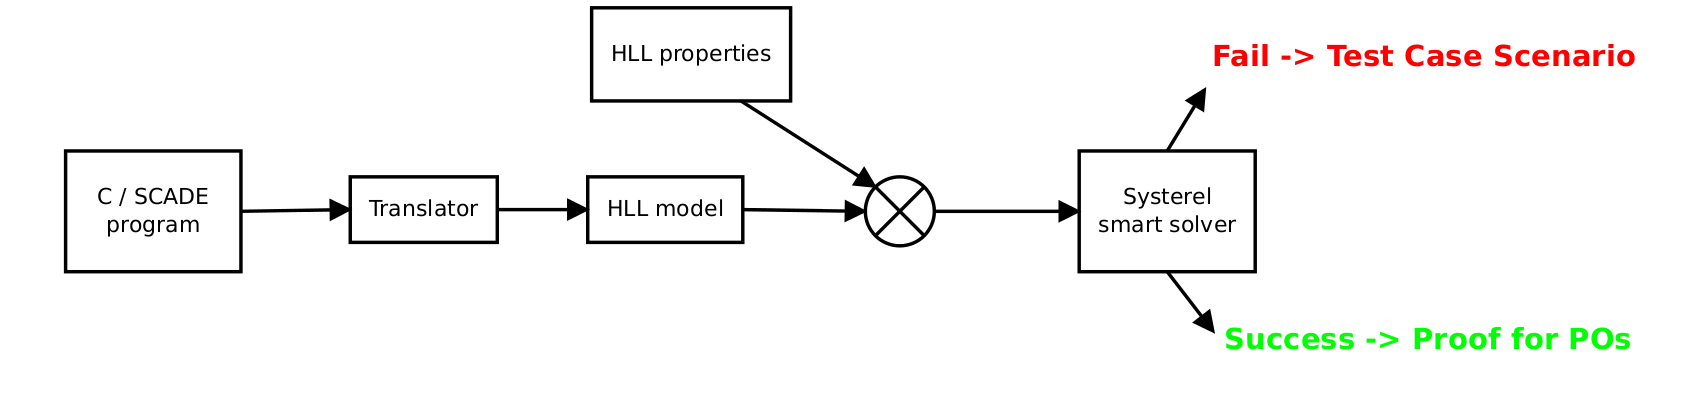
\includegraphics[width=1\textwidth]{S3_process}
\caption{Procedure of verification of Scade model}
\label{fig:procos}
\end{figure}

Figure \ref{fig:procos} describes the process:
\begin{itemize}
\item the main input is a Scade model to  verify (same approach and tool can be applied to a C program) which is translated in a High Level Language (a textual description of the model)
\item the second input is the propreties to verify, written in HLL
\item these both inputs are merged in aunique HLL file, used directly as input of the Systerel Smart Solver (S3 model-checker) for verification
\item result of the S3 tool is Success or Failure; in case of failure counter-example is provided for analyse.
\end{itemize}

The S3 tool is a model-checker which manages as well an internal SATs solver as external SAT solvers.

This process can be apply to cover three purposes:


\paragraph{ Properties of an HLL Model: } The prover may be used to prove or disprove properties of an HLL model. Those properties are modeled as proof obligations.
\begin{figure}[h!]
\centering
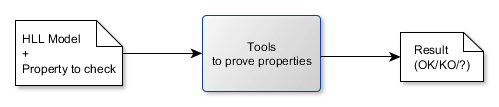
\includegraphics[width=1\textwidth]{Use_property_checker}
\caption{Properties of an HLL Model}
\label{fig:proch}
\end{figure}

\paragraph{ Solving Properties of an HLL Model: } The prover may be used as a solver, by finding values for the streams that comply with some property P. To do so, just put the negation of P as a proof obligation. If the prover succeeds to disprove the proof obligation, it will provide a solution solving P. If the prover succeeds to prove the proof obligation, then this proves that the property cannot be solved.
\begin{figure}[h!]
\centering
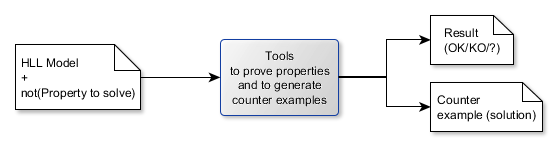
\includegraphics[width=1\textwidth]{Use_property_solver}
\caption{Solving Properties of an HLL Model}
\label{fig:prosolv}
\end{figure}

\paragraph{ Proving the Equivalence of 2 HLL Models: } The prover may be used to prove that 2 HLL models with the same interface (the same input streams and output streams) are equivalent. To do so, an equivalent model is produced with proof obligations stating that for all input streams values, each output of the first HLL model is equal to the output of the second model with the same name.
\begin{figure}[h!]
\centering
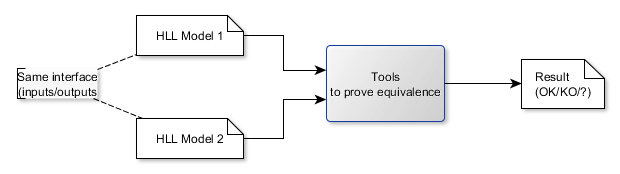
\includegraphics[width=1\textwidth]{Use_equivalence_checker}
\caption{Proving the Equivalence of 2 HLL Models}
\label{fig:eqch}
\end{figure}


\section{Specified properties and results}

\subsection{Proof of simple properties}


At first, the formal verification of the model was used to find bugs in the developed
Scade model.
A set of basic properties are automatically verified to check the well definition
of the Scade model: non-zero division, overflow, underflow, data range check,
initialization check,...

Then as we are focusing on sub-functions it is difficult to identify safety properties
to check on the whole model.

\subsubsection{Well definition of previous level}

\paragraph{Files used for the proof} The proof is defined in the file \url{https://github.com/openETCS/validation/blob/master/VnVUserStories/VnVUserStorySysterel/05-Work/S3/Proof_SoM/shunting_initiated_by_driver.hll} and it is verified on the top node \emph{xxx} of the Scade model \emph{Level Management}.

\paragraph{What is proved ?}


\paragraph{Constraints used}


\paragraph{Results}

\subsubsection{Conditions to Isolate mode}


\paragraph{Files used for the proof} The proof is defined in the file \url{https://github.com/openETCS/validation/blob/master/VnVUserStories/VnVUserStorySysterel/05-Work/S3/Proof_SoM/xxx} and it is verified on the top node \emph{xxx} of the Scade model \emph{Modes Management}.


\paragraph{What is proved ?}


\paragraph{Constraints used}


\paragraph{Results}

\subsection{Verification of use case}

\emph{levels}


\paragraph{Files used for the proof} The proof is defined in the file \url{https://github.com/openETCS/validation/blob/master/VnVUserStories/VnVUserStorySysterel/05-Work/S3/Proof_SoM/shunting_initiated_by_driver.hll} and it is verified on the top node \emph{xxx} of the Scade model \emph{Level Management}.

\paragraph{What is proved ?}


\paragraph{Constraints used}


\paragraph{Results}


\subsection{Validation of informal specification}

\subsubsection{Procedure Shunting initiated by Driver}

\paragraph{Files used for the proof} The proof is defined in the file \url{https://github.com/openETCS/validation/blob/master/VnVUserStories/VnVUserStorySysterel/05-Work/S3/Proof_SoM/shunting_initiated_by_driver.hll} and it is verified on the top node \emph{SH\_Initiated\_By\_Driver} of the Scade model \emph{Modes Management}.

\paragraph{What is proved ?}
We want to prove that the procedure SH\_Initiated\_By\_Driver is a
correct implementation of the section 5.6 Shunting Initiated By Driver of SRS-26.

To prove this, a specification of the flowchart is proposed in the
property file. However, the flowchart is not entirely specified:
elements \texttt{D030}, \texttt{A030}, \texttt{A095}, \texttt{S100} and
\texttt{A115} of the flow chart in SRS-26 are out of the scope of the mode management function.

\paragraph{Constraints used}
One hypothesis is used in this model to avoid a counter-example: when we are in \texttt{A100} the request of ``End of
Mission'' procedure correspond to the value of the input
\texttt{On-going Mission} as it is specified in the Scade model.

This hypothesis is justified by the fact that, according to
\texttt{A050}, \texttt{D040} and \texttt{A100}, if the input
\texttt{On-going Mission} is \texttt{True} then the ``End of Mission''
request is \texttt{True}, so equal to \texttt{On-going Mission}. Also,
as transition to SH mode is enable (\texttt{A050}) when ``End of
Mission'' request is made, the system should go to SH mode (or another
mode except SB mode). 

\paragraph{Results}
Considering the constraint and our model, the Scade model of
SH\_Initiated\_By\_Driver corresponds to the specification. Proof of this property allow to detect an error in Scade model: operator \emph{AND} was used instead operator \emph{OR}.
Besides the specification in Scade  of the computation of the output \emph{End\_Of\_Mission} was corrected.

\subsubsection{Procedure Start of Mission}

\paragraph{Files used for the proof}
The proof is defined in the file \url{https://github.com/openETCS/validation/blob/master/VnVUserStories/VnVUserStorySysterel/05-Work/S3/Proof_SoM/startofmission_topnode_proof.hll} and it is verified on the top node \emph{ManageModes} of the Scade model \emph{Modes Management}.


\paragraph{What is proved ?}
We want to prove that the procedure Procedure\_StartOfMission is a
correct implementation of the section 5.6 Procedure Start of mission of SRS-26.

Only the down part of the flowchart, from S10 and from S20, relative to the modes management, is specified in the Scade model.





\paragraph{Constraints used}
\begin{enumerate}
\item Level should not change : Level can be change at the beginning of Start of Mission procedure, but when we go in the step of mode selection, the level should not change.

\item Train Data should not change : Train Data are validated at the beginning of Start of Mission procedure, they shall be valid to start mode selection and we consider then that  their validity should not change.

\item The train shall stay at standstill during all the procedure. Indeed in Stand-By mode, standstill shall be ensure by supervision function (see SRS-26 §4.4.7.1.5).

\item The ``On Going Mission'' variable, input of SH Initiated by Driver, is
forced to False. This is justified by SRS 5, section ``5.4.6 Entry to
Mode Considered as a Mission''.
\end{enumerate}



\paragraph{Results}
Considering constraints and our hll model, the Scade model of Procedure
Start of Mission corresponds to the specification.
Some errors have been detected in the Scade model: links between nodes were wrong.

\subsubsection{Procedure On-Sight}
\emph{On going work}


\paragraph{Files used for the proof} The proof is defined in the file \url{https://github.com/openETCS/validation/blob/master/VnVUserStories/VnVUserStorySysterel/05-Work/S3/Proof_SoM/xxx} and it is verified on the top node \emph{xxx} of the Scade model \emph{Modes Management}.

\paragraph{What is proved ?}


\paragraph{Constraints used}


\paragraph{Results}


\subsection{Comparison of Scade models}

\emph{levels}\\
\\

\paragraph{Files used for the proof} The proof is defined in the file \url{https://github.com/openETCS/validation/blob/master/VnVUserStories/VnVUserStorySysterel/05-Work/S3/Proof_SoM/shunting_initiated_by_driver.hll} and it is verified on the top node \emph{xxx} of the Scade model \emph{Level Management}.

\paragraph{What is proved ?}


\paragraph{Constraints used}


\paragraph{Results}


\section{Conclusion}


\end{document}